% !TeX root = paper.tex
% Formato: ACM sigconf (dos columnas). Objetivo: 8 páginas de cuerpo; bibliografía aparte.
% Plantilla de clase: ./paper template/  ·  Bibliografía: ./references.bib
\PassOptionsToPackage{spanish,es-noshorthands}{babel}

\documentclass[sigconf, nonacm, language=spanish]{acmart}

\usepackage{tikz}
\usetikzlibrary{positioning,arrows.meta,fit,backgrounds,calc,bending}
% TikZ figures for paper.tex — compile via % TikZ figures for paper.tex — compile via % TikZ figures for paper.tex — compile via \input{figures/paper-figures}

\definecolor{sfclient}{RGB}{230,245,242}
\definecolor{sfserver}{RGB}{255,243,230}
\definecolor{sfgraph}{RGB}{238,232,248}
\definecolor{sfstore}{RGB}{242,242,242}
\definecolor{sfaccent}{RGB}{55,55,55}

\tikzset{
  sf/.style={font=\sffamily\footnotesize, text=sfaccent},
  sfbox/.style 2 args={
    sf, draw=#1, fill=#2, line width=0.6pt, rounded corners=2.5pt,
    align=center, inner sep=5pt, minimum height=0.78cm
  },
  sfarr/.style={-{Stealth[length=2.4mm,width=1.8mm]}, line width=0.7pt, draw=black!55},
  sfdarr/.style={sfarr, dashed, draw=black!40},
  sflbl/.style={sf, font=\scriptsize, fill=white, inner sep=1.5pt, text=black!65},
  sfphase/.style={
    draw=black!22, line width=0.5pt, dashed, rounded corners=4pt, inner sep=7pt
  },
  sfphaselabel/.style={sf, font=\scriptsize\bfseries, text=black!75},
}

\newcommand{\ArchitectureFigure}{%
  \begin{tikzpicture}[sf, node distance=0.5cm and 0.65cm]
    % Cliente (izquierda)
    \node[sfbox={teal!70}{sfclient}, minimum width=2.7cm] (ui) {Interfaz\\texto / voz};
    \node[sfbox={teal!70}{sfclient}, minimum width=2.7cm, below=of ui] (avatar) {Avatar VRM};
    \node[sfbox={teal!70}{sfclient}, minimum width=1.25cm, below left=0.4cm and 0cm of avatar] (stt) {Whisper};
    \node[sfbox={teal!70}{sfclient}, minimum width=1.25cm, below right=0.4cm and 0cm of avatar] (tts) {Edge-TTS};

    % API (centro)
    \node[sfbox={orange!75}{sfserver}, minimum width=2.0cm, right=1.4cm of avatar] (api) {FastAPI};
    \node[sf, font=\scriptsize, below=0.04cm of api] {REST + WebSocket};

    % LangGraph (derecha)
    \node[sfbox={violet!65}{sfgraph}, minimum width=2.6cm, right=1.2cm of api] (lg) {LangGraph};
    \node[sfbox={violet!65}{sfgraph}, minimum width=1.2cm, above left=0.3cm and -0.5cm of lg] (train) {Entren.};
    \node[sfbox={violet!65}{sfgraph}, minimum width=1.2cm, above=0.3cm of lg] (refine) {Refin.};
    \node[sfbox={violet!65}{sfgraph}, minimum width=1.2cm, above right=0.3cm and -0.5cm of lg] (valid) {Valid.};
    \node[sfbox={violet!65}{sfgraph}, minimum width=1.2cm, below=0.3cm of lg] (chat) {Chat A/B};

    % Infraestructura
    \node[sfbox={black!45}{sfstore}, minimum width=1.5cm, below left=0.55cm and 0.2cm of chat] (ollama) {Ollama};
    \node[sfbox={black!45}{sfstore}, minimum width=1.5cm, below=0.55cm of chat] (db) {SQLite};
    \node[sfbox={black!45}{sfstore}, minimum width=1.5cm, below right=0.55cm and 0.2cm of chat] (yaml) {Perfiles\\YAML};

    % Marcos de capa
    \node[sfphase, fit=(ui)(avatar)(stt)(tts),
      label={[sfphaselabel]above:Cliente Godot}] {};
    \node[sfphase, fit=(train)(refine)(valid)(chat)(lg)(ollama)(db)(yaml),
      label={[sfphaselabel]above:Backend Python}] {};

    % Conexiones
    \draw[sfarr] (ui.east) -- node[sflbl, above, pos=0.55] {WS} (api.west);
    \draw[sfarr] (avatar.east) -- (api.west);
    \draw[sfarr] (stt.east) -| ([yshift=0.15cm]api.south west);
    \draw[sfarr] (tts.east) -| ([yshift=0.15cm]api.south east);
    \draw[sfarr] (api.east) -- (lg.west);
    \draw[sfarr] (chat.south) -- (ollama.north);
    \draw[sfarr] (chat.south) -- (db.north);
    \draw[sfarr] (chat.south) -- (yaml.north);
    \draw[sfdarr] (train.south) -- (lg.north);
    \draw[sfdarr] (refine.south) -- (lg.north);
    \draw[sfdarr] (valid.south) -- (lg.north);
  \end{tikzpicture}%
}

\newcommand{\PipelineFigure}{%
  \begin{tikzpicture}[sf, node distance=0.42cm]
    \node[sfbox={blue!65}{blue!6}, minimum width=1.4cm] (in) {Entrada\\usuario};
    \node[sfbox={violet!65}{sfgraph}, minimum width=1.4cm, right=of in] (cls) {Clasificar\\situación};
    \node[sfbox={violet!65}{sfgraph}, minimum width=1.4cm, right=of cls] (ret) {Recuperar\\contexto};
    \node[sfbox={violet!65}{sfgraph}, minimum width=1.4cm, right=of ret] (plan) {Planificar\\conducta};
    \node[sfbox={violet!65}{sfgraph}, minimum width=1.4cm, right=of plan] (gen) {Generar\\respuesta};
    \node[sfbox={teal!70}{sfclient}, minimum width=1.4cm, right=of gen] (out) {Salida\\agente};

    \node[sfbox={black!45}{sfstore}, minimum width=1.15cm, below=0.7cm of ret] (yaml) {Perfil\\YAML};
    \node[sfbox={black!45}{sfstore}, minimum width=1.15cm, below=0.7cm of plan] (mom) {Momentos};

    \foreach \a/\b in {in/cls, cls/ret, ret/plan, plan/gen, gen/out}
      \draw[sfarr] (\a) -- (\b);

    \draw[sfdarr] (yaml.north) -- (ret.south);
    \draw[sfdarr] (mom.north) -- (plan.south);
    \draw[sfdarr] (yaml.east) -| (gen.south);

    \node[sf, font=\scriptsize\itshape, text=violet!70!black, below=0.08cm of cls] {solo A};
    \node[sf, font=\scriptsize\itshape, text=violet!70!black, below=0.08cm of ret] {solo A};
    \node[sf, font=\scriptsize\itshape, text=violet!70!black, below=0.08cm of plan] {solo A};

    \node[sfphase, fill=violet!3, fit=(cls)(ret)(plan)(gen),
      label={[sf, font=\scriptsize]above:Condición A}] {};
  \end{tikzpicture}%
}

\newcommand{\ProtocolFigure}{%
  \begin{tikzpicture}[sf, node distance=0.34cm and 0.32cm]
    % Fase 1
    \node[sfbox={orange!75}{sfserver}, minimum width=1.7cm] (t) {Entrenamiento};
    \node[sfbox={orange!75}{sfserver}, minimum width=1.7cm, right=of t] (r) {Refinamiento};
    \node[sfbox={orange!75}{sfserver}, minimum width=1.7cm, right=of r] (v) {Validación};
    \node[sf, font=\scriptsize\bfseries, right=0.15cm of v, text=orange!80!black] (ok) {$\geq$ umbrales};

    % Fase 2
    \node[sfbox={teal!70}{sfclient}, minimum width=1.55cm, below=1.2cm of t] (a) {Interacción A};
    \node[sfbox={teal!70}{sfclient}, minimum width=1.55cm, right=of a] (qa) {Cuestionario};
    \node[sfbox={teal!70}{sfclient}, minimum width=1.55cm, right=of qa] (b) {Interacción B};
    \node[sfbox={teal!70}{sfclient}, minimum width=1.55cm, right=of b] (qb) {Cuestionario};
    \node[sfbox={teal!70}{sfclient}, minimum width=1.55cm, right=of qb] (i) {Entrevista};

    % Contrabalanceo
    \node[sfbox={black!40}{sfstore}, minimum width=1.35cm, below=0.6cm of a] (ord1) {A$\rightarrow$B};
    \node[sfbox={black!40}{sfstore}, minimum width=1.35cm, below=0.6cm of b] (ord2) {B$\rightarrow$A};

    \node[sfphase, fill=orange!5, fit=(t)(r)(v)(ok),
      label={[sfphaselabel]above left:Fase 1 --- validación de perfil}] {};
    \node[sfphase, fill=teal!5, fit=(a)(qa)(b)(qb)(i)(ord1)(ord2),
      label={[sfphaselabel]above left:Fase 2 --- estudio piloto}] {};

    \draw[sfarr] (t) -- (r);
    \draw[sfarr] (r) -- (v);
    \draw[sfarr] (v) -- (ok);
    \draw[sfarr] (r.west) to[bend left=40] node[sflbl, above, pos=0.5] {si falla} (t.south);

    \draw[sfarr] (v.south) -- ++(0,-0.28) -| (a.north);

    \draw[sfarr] (a) -- (qa);
    \draw[sfarr] (qa) -- (b);
    \draw[sfarr] (b) -- (qb);
    \draw[sfarr] (qb) -- (i);

    \draw[sfdarr] (ord1.north) -- (a.south);
    \draw[sfdarr] (ord2.north) -- (b.south);
  \end{tikzpicture}%
}

\newcommand{\ManipulationFigure}{%
  \begin{tikzpicture}[sf, node distance=0.55cm]
    \node[sfbox={black!40}{sfstore}, minimum width=6.8cm, minimum height=0.65cm] (const)
      {Constantes: avatar \textbullet{} voz \textbullet{} interfaz \textbullet{} escenario \textbullet{} 5 min};

    \node[sfbox={teal!70}{sfclient}, minimum width=3.0cm, below left=0.75cm and -0.15cm of const] (a)
      {Condición A\\{\scriptsize perfil conductual}};
    \node[sfbox={orange!75}{sfserver}, minimum width=3.0cm, below right=0.75cm and -0.15cm of const] (b)
      {Condición B\\{\scriptsize control genérico}};

    \node[sf, align=center, font=\scriptsize, below=0.3cm of a, text width=3.1cm] {%
      Clasificación, recuperación\\y planificación activas};
    \node[sf, align=center, font=\scriptsize, below=0.3cm of b, text width=3.1cm] {%
      Sin pila conductual;\\prompt neutro};

    \draw[sfarr] (const.south west) -- (a.north);
    \draw[sfarr] (const.south east) -- (b.north);
  \end{tikzpicture}%
}

\newcommand{\DialogueFigure}{%
  \begin{tikzpicture}[sf]
    \node[sfbox={black!40}{sfstore}, minimum width=6.6cm, align=left, text width=6.2cm] (user) {%
      \textbf{Usuario:} Hola, hoy estuvo pesado en la u, llegué reventado.};
    \node[sfbox={teal!70}{sfclient}, minimum width=6.6cm, align=left, text width=6.2cm,
      below=0.45cm of user] (ca) {%
      \textbf{Condición A:} Ay, qué sorpresa, otro día fatal. ¿Y tú también sobreviviendo o qué?};
    \node[sfbox={orange!75}{sfserver}, minimum width=6.6cm, align=left, text width=6.2cm,
      below=0.45cm of ca] (cb) {%
      \textbf{Condición B:} Suena agotador. ¿Quieres contarme qué fue lo más pesado del día?};

    \node[sf, font=\scriptsize\itshape, below=0.12cm of cb, text=black!55]
      {Ilustración del sistema; no constituye dato experimental.};
  \end{tikzpicture}%
}


\definecolor{sfclient}{RGB}{230,245,242}
\definecolor{sfserver}{RGB}{255,243,230}
\definecolor{sfgraph}{RGB}{238,232,248}
\definecolor{sfstore}{RGB}{242,242,242}
\definecolor{sfaccent}{RGB}{55,55,55}

\tikzset{
  sf/.style={font=\sffamily\footnotesize, text=sfaccent},
  sfbox/.style 2 args={
    sf, draw=#1, fill=#2, line width=0.6pt, rounded corners=2.5pt,
    align=center, inner sep=5pt, minimum height=0.78cm
  },
  sfarr/.style={-{Stealth[length=2.4mm,width=1.8mm]}, line width=0.7pt, draw=black!55},
  sfdarr/.style={sfarr, dashed, draw=black!40},
  sflbl/.style={sf, font=\scriptsize, fill=white, inner sep=1.5pt, text=black!65},
  sfphase/.style={
    draw=black!22, line width=0.5pt, dashed, rounded corners=4pt, inner sep=7pt
  },
  sfphaselabel/.style={sf, font=\scriptsize\bfseries, text=black!75},
}

\newcommand{\ArchitectureFigure}{%
  \begin{tikzpicture}[sf, node distance=0.5cm and 0.65cm]
    % Cliente (izquierda)
    \node[sfbox={teal!70}{sfclient}, minimum width=2.7cm] (ui) {Interfaz\\texto / voz};
    \node[sfbox={teal!70}{sfclient}, minimum width=2.7cm, below=of ui] (avatar) {Avatar VRM};
    \node[sfbox={teal!70}{sfclient}, minimum width=1.25cm, below left=0.4cm and 0cm of avatar] (stt) {Whisper};
    \node[sfbox={teal!70}{sfclient}, minimum width=1.25cm, below right=0.4cm and 0cm of avatar] (tts) {Edge-TTS};

    % API (centro)
    \node[sfbox={orange!75}{sfserver}, minimum width=2.0cm, right=1.4cm of avatar] (api) {FastAPI};
    \node[sf, font=\scriptsize, below=0.04cm of api] {REST + WebSocket};

    % LangGraph (derecha)
    \node[sfbox={violet!65}{sfgraph}, minimum width=2.6cm, right=1.2cm of api] (lg) {LangGraph};
    \node[sfbox={violet!65}{sfgraph}, minimum width=1.2cm, above left=0.3cm and -0.5cm of lg] (train) {Entren.};
    \node[sfbox={violet!65}{sfgraph}, minimum width=1.2cm, above=0.3cm of lg] (refine) {Refin.};
    \node[sfbox={violet!65}{sfgraph}, minimum width=1.2cm, above right=0.3cm and -0.5cm of lg] (valid) {Valid.};
    \node[sfbox={violet!65}{sfgraph}, minimum width=1.2cm, below=0.3cm of lg] (chat) {Chat A/B};

    % Infraestructura
    \node[sfbox={black!45}{sfstore}, minimum width=1.5cm, below left=0.55cm and 0.2cm of chat] (ollama) {Ollama};
    \node[sfbox={black!45}{sfstore}, minimum width=1.5cm, below=0.55cm of chat] (db) {SQLite};
    \node[sfbox={black!45}{sfstore}, minimum width=1.5cm, below right=0.55cm and 0.2cm of chat] (yaml) {Perfiles\\YAML};

    % Marcos de capa
    \node[sfphase, fit=(ui)(avatar)(stt)(tts),
      label={[sfphaselabel]above:Cliente Godot}] {};
    \node[sfphase, fit=(train)(refine)(valid)(chat)(lg)(ollama)(db)(yaml),
      label={[sfphaselabel]above:Backend Python}] {};

    % Conexiones
    \draw[sfarr] (ui.east) -- node[sflbl, above, pos=0.55] {WS} (api.west);
    \draw[sfarr] (avatar.east) -- (api.west);
    \draw[sfarr] (stt.east) -| ([yshift=0.15cm]api.south west);
    \draw[sfarr] (tts.east) -| ([yshift=0.15cm]api.south east);
    \draw[sfarr] (api.east) -- (lg.west);
    \draw[sfarr] (chat.south) -- (ollama.north);
    \draw[sfarr] (chat.south) -- (db.north);
    \draw[sfarr] (chat.south) -- (yaml.north);
    \draw[sfdarr] (train.south) -- (lg.north);
    \draw[sfdarr] (refine.south) -- (lg.north);
    \draw[sfdarr] (valid.south) -- (lg.north);
  \end{tikzpicture}%
}

\newcommand{\PipelineFigure}{%
  \begin{tikzpicture}[sf, node distance=0.42cm]
    \node[sfbox={blue!65}{blue!6}, minimum width=1.4cm] (in) {Entrada\\usuario};
    \node[sfbox={violet!65}{sfgraph}, minimum width=1.4cm, right=of in] (cls) {Clasificar\\situación};
    \node[sfbox={violet!65}{sfgraph}, minimum width=1.4cm, right=of cls] (ret) {Recuperar\\contexto};
    \node[sfbox={violet!65}{sfgraph}, minimum width=1.4cm, right=of ret] (plan) {Planificar\\conducta};
    \node[sfbox={violet!65}{sfgraph}, minimum width=1.4cm, right=of plan] (gen) {Generar\\respuesta};
    \node[sfbox={teal!70}{sfclient}, minimum width=1.4cm, right=of gen] (out) {Salida\\agente};

    \node[sfbox={black!45}{sfstore}, minimum width=1.15cm, below=0.7cm of ret] (yaml) {Perfil\\YAML};
    \node[sfbox={black!45}{sfstore}, minimum width=1.15cm, below=0.7cm of plan] (mom) {Momentos};

    \foreach \a/\b in {in/cls, cls/ret, ret/plan, plan/gen, gen/out}
      \draw[sfarr] (\a) -- (\b);

    \draw[sfdarr] (yaml.north) -- (ret.south);
    \draw[sfdarr] (mom.north) -- (plan.south);
    \draw[sfdarr] (yaml.east) -| (gen.south);

    \node[sf, font=\scriptsize\itshape, text=violet!70!black, below=0.08cm of cls] {solo A};
    \node[sf, font=\scriptsize\itshape, text=violet!70!black, below=0.08cm of ret] {solo A};
    \node[sf, font=\scriptsize\itshape, text=violet!70!black, below=0.08cm of plan] {solo A};

    \node[sfphase, fill=violet!3, fit=(cls)(ret)(plan)(gen),
      label={[sf, font=\scriptsize]above:Condición A}] {};
  \end{tikzpicture}%
}

\newcommand{\ProtocolFigure}{%
  \begin{tikzpicture}[sf, node distance=0.34cm and 0.32cm]
    % Fase 1
    \node[sfbox={orange!75}{sfserver}, minimum width=1.7cm] (t) {Entrenamiento};
    \node[sfbox={orange!75}{sfserver}, minimum width=1.7cm, right=of t] (r) {Refinamiento};
    \node[sfbox={orange!75}{sfserver}, minimum width=1.7cm, right=of r] (v) {Validación};
    \node[sf, font=\scriptsize\bfseries, right=0.15cm of v, text=orange!80!black] (ok) {$\geq$ umbrales};

    % Fase 2
    \node[sfbox={teal!70}{sfclient}, minimum width=1.55cm, below=1.2cm of t] (a) {Interacción A};
    \node[sfbox={teal!70}{sfclient}, minimum width=1.55cm, right=of a] (qa) {Cuestionario};
    \node[sfbox={teal!70}{sfclient}, minimum width=1.55cm, right=of qa] (b) {Interacción B};
    \node[sfbox={teal!70}{sfclient}, minimum width=1.55cm, right=of b] (qb) {Cuestionario};
    \node[sfbox={teal!70}{sfclient}, minimum width=1.55cm, right=of qb] (i) {Entrevista};

    % Contrabalanceo
    \node[sfbox={black!40}{sfstore}, minimum width=1.35cm, below=0.6cm of a] (ord1) {A$\rightarrow$B};
    \node[sfbox={black!40}{sfstore}, minimum width=1.35cm, below=0.6cm of b] (ord2) {B$\rightarrow$A};

    \node[sfphase, fill=orange!5, fit=(t)(r)(v)(ok),
      label={[sfphaselabel]above left:Fase 1 --- validación de perfil}] {};
    \node[sfphase, fill=teal!5, fit=(a)(qa)(b)(qb)(i)(ord1)(ord2),
      label={[sfphaselabel]above left:Fase 2 --- estudio piloto}] {};

    \draw[sfarr] (t) -- (r);
    \draw[sfarr] (r) -- (v);
    \draw[sfarr] (v) -- (ok);
    \draw[sfarr] (r.west) to[bend left=40] node[sflbl, above, pos=0.5] {si falla} (t.south);

    \draw[sfarr] (v.south) -- ++(0,-0.28) -| (a.north);

    \draw[sfarr] (a) -- (qa);
    \draw[sfarr] (qa) -- (b);
    \draw[sfarr] (b) -- (qb);
    \draw[sfarr] (qb) -- (i);

    \draw[sfdarr] (ord1.north) -- (a.south);
    \draw[sfdarr] (ord2.north) -- (b.south);
  \end{tikzpicture}%
}

\newcommand{\ManipulationFigure}{%
  \begin{tikzpicture}[sf, node distance=0.55cm]
    \node[sfbox={black!40}{sfstore}, minimum width=6.8cm, minimum height=0.65cm] (const)
      {Constantes: avatar \textbullet{} voz \textbullet{} interfaz \textbullet{} escenario \textbullet{} 5 min};

    \node[sfbox={teal!70}{sfclient}, minimum width=3.0cm, below left=0.75cm and -0.15cm of const] (a)
      {Condición A\\{\scriptsize perfil conductual}};
    \node[sfbox={orange!75}{sfserver}, minimum width=3.0cm, below right=0.75cm and -0.15cm of const] (b)
      {Condición B\\{\scriptsize control genérico}};

    \node[sf, align=center, font=\scriptsize, below=0.3cm of a, text width=3.1cm] {%
      Clasificación, recuperación\\y planificación activas};
    \node[sf, align=center, font=\scriptsize, below=0.3cm of b, text width=3.1cm] {%
      Sin pila conductual;\\prompt neutro};

    \draw[sfarr] (const.south west) -- (a.north);
    \draw[sfarr] (const.south east) -- (b.north);
  \end{tikzpicture}%
}

\newcommand{\DialogueFigure}{%
  \begin{tikzpicture}[sf]
    \node[sfbox={black!40}{sfstore}, minimum width=6.6cm, align=left, text width=6.2cm] (user) {%
      \textbf{Usuario:} Hola, hoy estuvo pesado en la u, llegué reventado.};
    \node[sfbox={teal!70}{sfclient}, minimum width=6.6cm, align=left, text width=6.2cm,
      below=0.45cm of user] (ca) {%
      \textbf{Condición A:} Ay, qué sorpresa, otro día fatal. ¿Y tú también sobreviviendo o qué?};
    \node[sfbox={orange!75}{sfserver}, minimum width=6.6cm, align=left, text width=6.2cm,
      below=0.45cm of ca] (cb) {%
      \textbf{Condición B:} Suena agotador. ¿Quieres contarme qué fue lo más pesado del día?};

    \node[sf, font=\scriptsize\itshape, below=0.12cm of cb, text=black!55]
      {Ilustración del sistema; no constituye dato experimental.};
  \end{tikzpicture}%
}


\definecolor{sfclient}{RGB}{230,245,242}
\definecolor{sfserver}{RGB}{255,243,230}
\definecolor{sfgraph}{RGB}{238,232,248}
\definecolor{sfstore}{RGB}{242,242,242}
\definecolor{sfaccent}{RGB}{55,55,55}

\tikzset{
  sf/.style={font=\sffamily\footnotesize, text=sfaccent},
  sfbox/.style 2 args={
    sf, draw=#1, fill=#2, line width=0.6pt, rounded corners=2.5pt,
    align=center, inner sep=5pt, minimum height=0.78cm
  },
  sfarr/.style={-{Stealth[length=2.4mm,width=1.8mm]}, line width=0.7pt, draw=black!55},
  sfdarr/.style={sfarr, dashed, draw=black!40},
  sflbl/.style={sf, font=\scriptsize, fill=white, inner sep=1.5pt, text=black!65},
  sfphase/.style={
    draw=black!22, line width=0.5pt, dashed, rounded corners=4pt, inner sep=7pt
  },
  sfphaselabel/.style={sf, font=\scriptsize\bfseries, text=black!75},
}

\newcommand{\ArchitectureFigure}{%
  \begin{tikzpicture}[sf, node distance=0.5cm and 0.65cm]
    % Cliente (izquierda)
    \node[sfbox={teal!70}{sfclient}, minimum width=2.7cm] (ui) {Interfaz\\texto / voz};
    \node[sfbox={teal!70}{sfclient}, minimum width=2.7cm, below=of ui] (avatar) {Avatar VRM};
    \node[sfbox={teal!70}{sfclient}, minimum width=1.25cm, below left=0.4cm and 0cm of avatar] (stt) {Whisper};
    \node[sfbox={teal!70}{sfclient}, minimum width=1.25cm, below right=0.4cm and 0cm of avatar] (tts) {Edge-TTS};

    % API (centro)
    \node[sfbox={orange!75}{sfserver}, minimum width=2.0cm, right=1.4cm of avatar] (api) {FastAPI};
    \node[sf, font=\scriptsize, below=0.04cm of api] {REST + WebSocket};

    % LangGraph (derecha)
    \node[sfbox={violet!65}{sfgraph}, minimum width=2.6cm, right=1.2cm of api] (lg) {LangGraph};
    \node[sfbox={violet!65}{sfgraph}, minimum width=1.2cm, above left=0.3cm and -0.5cm of lg] (train) {Entren.};
    \node[sfbox={violet!65}{sfgraph}, minimum width=1.2cm, above=0.3cm of lg] (refine) {Refin.};
    \node[sfbox={violet!65}{sfgraph}, minimum width=1.2cm, above right=0.3cm and -0.5cm of lg] (valid) {Valid.};
    \node[sfbox={violet!65}{sfgraph}, minimum width=1.2cm, below=0.3cm of lg] (chat) {Chat A/B};

    % Infraestructura
    \node[sfbox={black!45}{sfstore}, minimum width=1.5cm, below left=0.55cm and 0.2cm of chat] (ollama) {Ollama};
    \node[sfbox={black!45}{sfstore}, minimum width=1.5cm, below=0.55cm of chat] (db) {SQLite};
    \node[sfbox={black!45}{sfstore}, minimum width=1.5cm, below right=0.55cm and 0.2cm of chat] (yaml) {Perfiles\\YAML};

    % Marcos de capa
    \node[sfphase, fit=(ui)(avatar)(stt)(tts),
      label={[sfphaselabel]above:Cliente Godot}] {};
    \node[sfphase, fit=(train)(refine)(valid)(chat)(lg)(ollama)(db)(yaml),
      label={[sfphaselabel]above:Backend Python}] {};

    % Conexiones
    \draw[sfarr] (ui.east) -- node[sflbl, above, pos=0.55] {WS} (api.west);
    \draw[sfarr] (avatar.east) -- (api.west);
    \draw[sfarr] (stt.east) -| ([yshift=0.15cm]api.south west);
    \draw[sfarr] (tts.east) -| ([yshift=0.15cm]api.south east);
    \draw[sfarr] (api.east) -- (lg.west);
    \draw[sfarr] (chat.south) -- (ollama.north);
    \draw[sfarr] (chat.south) -- (db.north);
    \draw[sfarr] (chat.south) -- (yaml.north);
    \draw[sfdarr] (train.south) -- (lg.north);
    \draw[sfdarr] (refine.south) -- (lg.north);
    \draw[sfdarr] (valid.south) -- (lg.north);
  \end{tikzpicture}%
}

\newcommand{\PipelineFigure}{%
  \begin{tikzpicture}[sf, node distance=0.42cm]
    \node[sfbox={blue!65}{blue!6}, minimum width=1.4cm] (in) {Entrada\\usuario};
    \node[sfbox={violet!65}{sfgraph}, minimum width=1.4cm, right=of in] (cls) {Clasificar\\situación};
    \node[sfbox={violet!65}{sfgraph}, minimum width=1.4cm, right=of cls] (ret) {Recuperar\\contexto};
    \node[sfbox={violet!65}{sfgraph}, minimum width=1.4cm, right=of ret] (plan) {Planificar\\conducta};
    \node[sfbox={violet!65}{sfgraph}, minimum width=1.4cm, right=of plan] (gen) {Generar\\respuesta};
    \node[sfbox={teal!70}{sfclient}, minimum width=1.4cm, right=of gen] (out) {Salida\\agente};

    \node[sfbox={black!45}{sfstore}, minimum width=1.15cm, below=0.7cm of ret] (yaml) {Perfil\\YAML};
    \node[sfbox={black!45}{sfstore}, minimum width=1.15cm, below=0.7cm of plan] (mom) {Momentos};

    \foreach \a/\b in {in/cls, cls/ret, ret/plan, plan/gen, gen/out}
      \draw[sfarr] (\a) -- (\b);

    \draw[sfdarr] (yaml.north) -- (ret.south);
    \draw[sfdarr] (mom.north) -- (plan.south);
    \draw[sfdarr] (yaml.east) -| (gen.south);

    \node[sf, font=\scriptsize\itshape, text=violet!70!black, below=0.08cm of cls] {solo A};
    \node[sf, font=\scriptsize\itshape, text=violet!70!black, below=0.08cm of ret] {solo A};
    \node[sf, font=\scriptsize\itshape, text=violet!70!black, below=0.08cm of plan] {solo A};

    \node[sfphase, fill=violet!3, fit=(cls)(ret)(plan)(gen),
      label={[sf, font=\scriptsize]above:Condición A}] {};
  \end{tikzpicture}%
}

\newcommand{\ProtocolFigure}{%
  \begin{tikzpicture}[sf, node distance=0.34cm and 0.32cm]
    % Fase 1
    \node[sfbox={orange!75}{sfserver}, minimum width=1.7cm] (t) {Entrenamiento};
    \node[sfbox={orange!75}{sfserver}, minimum width=1.7cm, right=of t] (r) {Refinamiento};
    \node[sfbox={orange!75}{sfserver}, minimum width=1.7cm, right=of r] (v) {Validación};
    \node[sf, font=\scriptsize\bfseries, right=0.15cm of v, text=orange!80!black] (ok) {$\geq$ umbrales};

    % Fase 2
    \node[sfbox={teal!70}{sfclient}, minimum width=1.55cm, below=1.2cm of t] (a) {Interacción A};
    \node[sfbox={teal!70}{sfclient}, minimum width=1.55cm, right=of a] (qa) {Cuestionario};
    \node[sfbox={teal!70}{sfclient}, minimum width=1.55cm, right=of qa] (b) {Interacción B};
    \node[sfbox={teal!70}{sfclient}, minimum width=1.55cm, right=of b] (qb) {Cuestionario};
    \node[sfbox={teal!70}{sfclient}, minimum width=1.55cm, right=of qb] (i) {Entrevista};

    % Contrabalanceo
    \node[sfbox={black!40}{sfstore}, minimum width=1.35cm, below=0.6cm of a] (ord1) {A$\rightarrow$B};
    \node[sfbox={black!40}{sfstore}, minimum width=1.35cm, below=0.6cm of b] (ord2) {B$\rightarrow$A};

    \node[sfphase, fill=orange!5, fit=(t)(r)(v)(ok),
      label={[sfphaselabel]above left:Fase 1 --- validación de perfil}] {};
    \node[sfphase, fill=teal!5, fit=(a)(qa)(b)(qb)(i)(ord1)(ord2),
      label={[sfphaselabel]above left:Fase 2 --- estudio piloto}] {};

    \draw[sfarr] (t) -- (r);
    \draw[sfarr] (r) -- (v);
    \draw[sfarr] (v) -- (ok);
    \draw[sfarr] (r.west) to[bend left=40] node[sflbl, above, pos=0.5] {si falla} (t.south);

    \draw[sfarr] (v.south) -- ++(0,-0.28) -| (a.north);

    \draw[sfarr] (a) -- (qa);
    \draw[sfarr] (qa) -- (b);
    \draw[sfarr] (b) -- (qb);
    \draw[sfarr] (qb) -- (i);

    \draw[sfdarr] (ord1.north) -- (a.south);
    \draw[sfdarr] (ord2.north) -- (b.south);
  \end{tikzpicture}%
}

\newcommand{\ManipulationFigure}{%
  \begin{tikzpicture}[sf, node distance=0.55cm]
    \node[sfbox={black!40}{sfstore}, minimum width=6.8cm, minimum height=0.65cm] (const)
      {Constantes: avatar \textbullet{} voz \textbullet{} interfaz \textbullet{} escenario \textbullet{} 5 min};

    \node[sfbox={teal!70}{sfclient}, minimum width=3.0cm, below left=0.75cm and -0.15cm of const] (a)
      {Condición A\\{\scriptsize perfil conductual}};
    \node[sfbox={orange!75}{sfserver}, minimum width=3.0cm, below right=0.75cm and -0.15cm of const] (b)
      {Condición B\\{\scriptsize control genérico}};

    \node[sf, align=center, font=\scriptsize, below=0.3cm of a, text width=3.1cm] {%
      Clasificación, recuperación\\y planificación activas};
    \node[sf, align=center, font=\scriptsize, below=0.3cm of b, text width=3.1cm] {%
      Sin pila conductual;\\prompt neutro};

    \draw[sfarr] (const.south west) -- (a.north);
    \draw[sfarr] (const.south east) -- (b.north);
  \end{tikzpicture}%
}

\newcommand{\DialogueFigure}{%
  \begin{tikzpicture}[sf]
    \node[sfbox={black!40}{sfstore}, minimum width=6.6cm, align=left, text width=6.2cm] (user) {%
      \textbf{Usuario:} Hola, hoy estuvo pesado en la u, llegué reventado.};
    \node[sfbox={teal!70}{sfclient}, minimum width=6.6cm, align=left, text width=6.2cm,
      below=0.45cm of user] (ca) {%
      \textbf{Condición A:} Ay, qué sorpresa, otro día fatal. ¿Y tú también sobreviviendo o qué?};
    \node[sfbox={orange!75}{sfserver}, minimum width=6.6cm, align=left, text width=6.2cm,
      below=0.45cm of ca] (cb) {%
      \textbf{Condición B:} Suena agotador. ¿Quieres contarme qué fue lo más pesado del día?};

    \node[sf, font=\scriptsize\itshape, below=0.12cm of cb, text=black!55]
      {Ilustración del sistema; no constituye dato experimental.};
  \end{tikzpicture}%
}


\settopmatter{printccs=false, printacmref=false}

\setcopyright{acmlicensed}
\copyrightyear{2026}
\acmYear{2026}
\acmDOI{XXXXXXX.XXXXXXX}
\acmConference[CI'26]{Conferencia por definir}{Mes DD--DD, 2026}{Ciudad, País}
\acmISBN{978-1-4503-XXXX-X/2026/XX}

\begin{document}

\title[Suena Familiar]{Suena Familiar: Percepción de Familiaridad en Agentes Virtuales Mediante Familiaridad Conductual}

\author{Luis Carlos Quesada Rodríguez}
\email{luiscarlos.quesada@ucr.ac.cr}
\affiliation{%
  \institution{Universidad de Costa Rica}
  \city{San José}
  \country{Costa Rica}
}

\begin{abstract}
  Los agentes conversacionales actuales pueden mantener interacciones naturales, pero rara vez evocan la sensación de estar conversando con alguien familiar. Aunque investigaciones previas han estudiado familiaridad mediante apariencia, voz o conocimiento contextual, existe poca evidencia sobre el papel de los patrones conductuales en la generación de esta percepción.

Este trabajo explora la familiaridad conductual como un mecanismo capaz de activar modelos mentales asociados a personas conocidas a partir de señales conversacionales implícitas. Para ello se propone una metodología de construcción, refinamiento y validación de perfiles conductuales, posteriormente utilizados dentro de un diseño experimental que compara una condición basada en familiaridad conductual con una condición conversacional genérica.

Un estudio piloto preliminar ($n=3$) sugiere que las señales conductuales pueden influir sobre la percepción de familiaridad, presencia social y conocimiento contextual percibido. Los resultados también indican que familiaridad y respuesta afectiva positiva no son necesariamente equivalentes. Aunque exploratorios, estos hallazgos apoyan la viabilidad de estudiar la familiaridad como un fenómeno conductual independiente de la apariencia o la identidad explícita en agentes virtuales.

    
\end{abstract}

\keywords{familiaridad conductual, modelos mentales, agentes conversacionales, interacción humano-computadora, presencia social, manipulación experimental}

\maketitle

\section{Introducción}

Los agentes conversacionales impulsados por modelos de lenguaje están evolucionando rápidamente desde asistentes orientados a tareas hacia interlocutores capaces de participar en interacciones cada vez más sociales. A medida que estos sistemas se incorporan a contextos educativos, laborales y personales, surge una pregunta fundamental: ¿qué hace que un agente se sienta socialmente familiar para un usuario?

La familiaridad es una señal social poderosa. Diversos trabajos han mostrado que puede orientar la atención, reducir la incertidumbre interpretativa y modular la disposición a confiar \cite{garciamarques_familiarity_2007, poletaykina_knowing_2025}. En la vida cotidiana, reconocemos el estilo conversacional de personas conocidas a partir de patrones sutiles de interacción: su ritmo, sus expresiones recurrentes, sus preferencias comunicativas o la forma en que desarrollan una conversación. Estas señales pueden resultar reconocibles incluso cuando no existe información visual o contextual suficiente para identificar explícitamente a la persona.

Sin embargo, los agentes conversacionales actuales rara vez generan este tipo de percepción \cite{yang_exploring_2025}. La literatura describe con detalle qué ocurre cuando un agente parece familiar, pero dedica menos atención a comprender cómo puede inducirse dicha familiaridad de manera controlada mediante el comportamiento conversacional por sí solo.

Este vacío resulta especialmente relevante porque gran parte de los enfoques existentes combinan familiaridad con otros mecanismos como apariencia visual, memoria persistente, voz sintética personalizada o representación explícita de identidad \cite{poletaykina_knowing_2025, yang_exploring_2025}. En consecuencia, resulta difícil determinar qué parte de la percepción observada corresponde realmente a la familiaridad y cuál responde a otros factores como reconocimiento facial, continuidad temporal o personalización declarada.

La propuesta de este trabajo aborda este problema desde una perspectiva distinta. En lugar de intentar reproducir a una persona específica o personalizar la interacción mediante información explícita del usuario, se introduce el concepto de \emph{familiaridad conductual}: la utilización de señales conversacionales capaces de activar modelos mentales asociados a personas conocidas sin recurrir a la reproducción de identidad, apariencia o voz. Desde esta perspectiva, el interés no reside en que el agente sea percibido como una persona concreta, sino en estudiar si determinados patrones de comportamiento son suficientes para evocar sensaciones de reconocimiento y familiaridad durante la interacción.

La contribución principal es metodológica. Se propone un procedimiento para construir, refinar y validar perfiles conductuales antes de su utilización dentro de un experimento controlado, permitiendo que la Condición A funcione como una manipulación creíble de familiaridad implícita frente a una condición de control con comportamiento genérico. Sobre esta base se desarrolla un estudio piloto orientado a explorar si dichas señales conductuales influyen sobre la percepción de familiaridad, presencia social, respuesta afectiva y conocimiento contextual percibido, utilizando instrumentos como Godspeed \cite{bartneck_measurement_2009}, SAM \cite{bradley_measures_1994} y escalas Likert.

El agente propuesto no intenta ser la persona modelada. Su objetivo es generar suficientes señales conductuales para que un observador familiarizado pueda percibir reconocimiento, familiaridad o conocimiento previo como resultado de la interacción. Esta distinción permite estudiar la familiaridad como un fenómeno conductual y perceptivo, independiente de mecanismos explícitos de identidad o representación visual.


\section{Trabajo Relacionado}

\subsection{Familiaridad y Modelos Mentales de Personas Conocidas}

La familiaridad constituye un mecanismo fundamental de la cognición humana. Dentro de las teorías de doble proceso de memoria, suele distinguirse de la evocación (\textit{recollection}), ya que permite experimentar una sensación de reconocimiento sin necesidad de recuperar conscientemente detalles contextuales asociados a experiencias previas \cite{mickes_recollection_2009}. Diversos trabajos han sugerido además que la familiaridad puede emerger a partir de procesos de fluidez cognitiva, donde estímulos previamente experimentados son procesados con mayor facilidad y, por tanto, percibidos como más familiares \cite{kelley_subjective_1998, mecklinger_fluency_2020}.

En contextos sociales, estas señales contribuyen a la construcción de modelos mentales sobre otras personas. Dichos modelos permiten anticipar comportamientos, interpretar intenciones y generar expectativas sobre futuras interacciones \cite{tamir_predicting_2024}. A medida que aumenta el conocimiento previo sobre un individuo, estos modelos se vuelven más ricos y detallados, incorporando patrones conversacionales, preferencias comunicativas y características conductuales recurrentes.

La presente investigación parte de la hipótesis de que ciertas señales conductuales podrían ser suficientes para activar parcialmente estos modelos mentales durante la interacción con un agente artificial. Desde esta perspectiva, el interés no reside en reproducir la identidad de una persona, sino en estudiar si determinados patrones conversacionales pueden evocar sensaciones de familiaridad asociadas a individuos conocidos.

\subsection{Familiaridad en Agentes Virtuales}

La familiaridad ha sido estudiada previamente en el contexto de agentes virtuales inteligentes y agentes relacionales. Investigaciones tempranas mostraron que la continuidad de interacción, la consistencia conductual y la capacidad de mantener relaciones a largo plazo pueden influir sobre la percepción social de los usuarios \cite{bickmore_relational_2001}. Trabajos posteriores sugieren que estas características pueden favorecer confianza, cercanía percibida y compromiso durante la interacción \cite{bickmore_relational_2001}.

Más recientemente, diversos autores han explorado mecanismos explícitos para generar familiaridad en agentes virtuales. Poletaykina et al.\ encontraron que agentes visualmente familiares pueden incrementar confianza y percepción positiva durante la interacción \cite{poletaykina_knowing_2025}. De manera similar, Yang et al.\ analizaron cómo familiaridad y conocimiento contextual percibido influyen sobre la percepción de agentes conversacionales, utilizando representaciones explícitas de personas conocidas y elementos visuales asociados a ellas \cite{yang_exploring_2025}.

Estos resultados sugieren que la familiaridad puede influir significativamente sobre la forma en que los usuarios interpretan y evalúan agentes virtuales. Sin embargo, la mayoría de las aproximaciones existentes combinan simultáneamente múltiples señales de familiaridad, incluyendo apariencia visual, identidad explícita, voz, memoria o conocimiento contextual, dificultando aislar el efecto específico de la conducta conversacional.

\subsection{Alineación Conversacional e Imitación Conductual}

La comunicación humana presenta fenómenos de alineación lingüística y acomodación conversacional mediante los cuales los interlocutores ajustan progresivamente patrones de comunicación durante una interacción \cite{branigan_linguistic_2010}. Estos mecanismos pueden manifestarse en vocabulario, estructuras sintácticas, longitud de respuestas o estrategias discursivas compartidas.

De manera similar, investigaciones sobre mimetismo e interacción social han mostrado que los individuos son sensibles a patrones sutiles de comportamiento durante la comunicación \cite{caridakis_virtual_2007}. Aunque estas estrategias pueden favorecer naturalidad y coherencia conversacional, también pueden generar respuestas negativas cuando el comportamiento percibido resulta excesivamente artificial o intrusivo \cite{wang_stop_2023}.

No obstante, gran parte de esta literatura estudia procesos de adaptación producidos dentro de la interacción misma. En contraste, el presente trabajo explora si patrones conductuales previamente asociados a una persona conocida pueden ser utilizados para evocar familiaridad antes de que exista una historia compartida entre usuario y agente.

\subsection{Posicionamiento de Este Trabajo}

La presente propuesta busca aislar la conducta conversacional como mecanismo principal de familiaridad. En lugar de utilizar apariencia visual, voz personalizada o representación explícita de identidad, el estudio explora si patrones conversacionales asociados a una persona conocida pueden activar modelos mentales preexistentes durante la interacción con un agente virtual.

La contribución central no consiste en desarrollar una réplica digital de una persona ni en maximizar semejanza con un individuo real. En su lugar, se propone una metodología para construir, refinar y validar perfiles conductuales antes de su utilización dentro de un experimento controlado. La validación previa de dichos perfiles funciona como un chequeo de manipulación experimental orientado a verificar que el perfil genera señales reconocibles de familiaridad antes de exponer participantes a la condición experimental.

Esta aproximación permite estudiar la familiaridad como un fenómeno conductual independiente de mecanismos explícitos de identidad, abordando una pregunta aún poco explorada en la literatura: ¿pueden patrones conversacionales por sí solos activar modelos mentales asociados a personas conocidas durante la interacción con un agente virtual?

\section{Diseño del Sistema}

El objetivo de la plataforma no consiste en reproducir digitalmente a una persona específica, sino en proporcionar un entorno controlado para estudiar familiaridad conductual como fenómeno experimental. Para ello, el sistema implementa mecanismos para construir, almacenar y utilizar perfiles conductuales capaces de influir sobre el comportamiento conversacional de un agente virtual, manteniendo constantes los demás elementos de interacción.

\subsection{Plataforma Experimental}

La plataforma fue desarrollada sobre Godot e integra interacción conversacional mediante texto y voz. El cliente gestiona la experiencia del participante, incluyendo la interfaz conversacional, el avatar virtual y la reproducción de audio. Por su parte, el backend coordina la generación conversacional, la síntesis de voz y la administración de perfiles conductuales.

La Figura~\ref{fig:architecture} presenta una visión general de la arquitectura utilizada. El sistema se diseñó de forma desacoplada para permitir la modificación de perfiles conductuales sin alterar los componentes de interacción percibidos por el usuario.

\begin{figure*}[t]
  \centering
  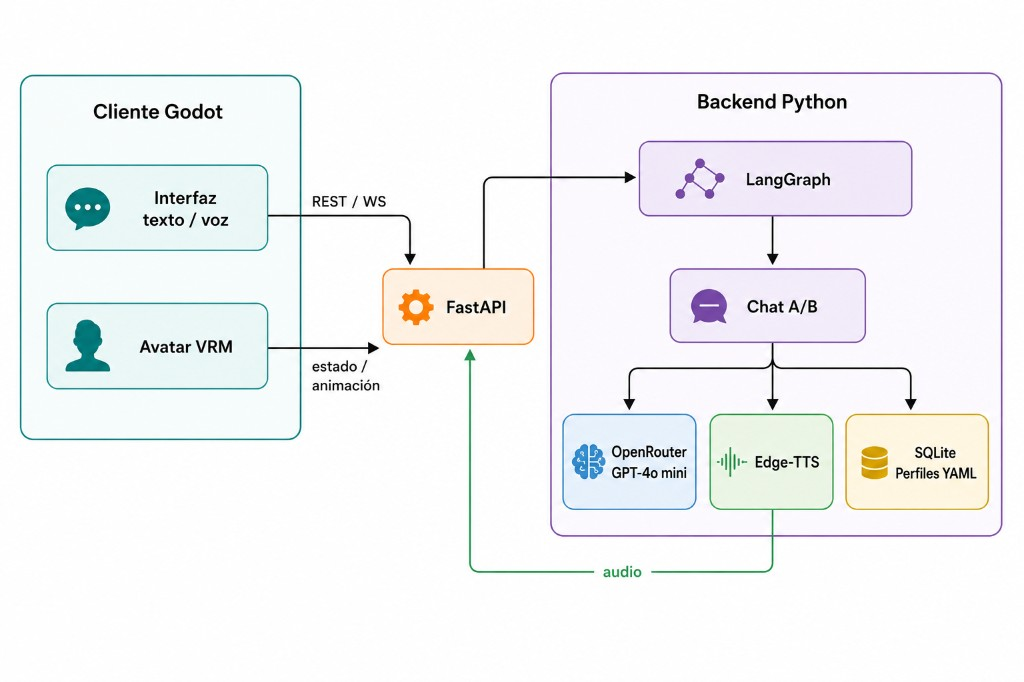
\includegraphics[width=\textwidth]{figures/architecture.png}
  \caption{Visión general de la plataforma experimental. El cliente Godot gestiona la interacción del participante; el backend coordina la generación conversacional, la síntesis de voz y los perfiles conductuales. Avatar, voz e interfaz permanecen constantes entre condiciones; solo cambia el perfil conductual activo.}
  \Description{Diagrama cliente-servidor: cliente Godot, backend conversacional, modelo de lenguaje, síntesis de voz y almacenamiento de perfiles.}
  \label{fig:architecture}
\end{figure*}

Aunque la arquitectura incorpora diversos componentes tecnológicos, el foco de la investigación no se encuentra en la evaluación técnica de la plataforma, sino en el estudio de los efectos perceptuales asociados a los perfiles conductuales utilizados por el agente.

\subsection{Perfiles Conductuales}

Los perfiles conductuales constituyen el mecanismo principal mediante el cual se implementa la familiaridad conductual dentro del sistema.

Cada perfil almacena patrones conversacionales, preferencias comunicativas, tendencias de estilo, restricciones de comportamiento y material contextual asociado a la persona modelada. Estos elementos son utilizados durante la generación de respuestas para modificar el comportamiento observable del agente sin alterar su representación visual o identidad explícita.

La construcción de los perfiles se basa en entrevistas conversacionales con la persona modelada, a partir de las cuales se identifican patrones recurrentes de comunicación, preferencias discursivas y características de estilo relevantes para la interacción.

Una vez generado un perfil inicial, este puede ser refinado iterativamente mediante retroalimentación de la persona modelada y posteriormente sometido a procesos de validación antes de su utilización dentro de evaluaciones experimentales.

\subsection{Validación de Perfiles}

Antes de ser utilizados dentro de sesiones experimentales, los perfiles conductuales son sometidos a un proceso de validación destinado a verificar que generan señales suficientemente consistentes de familiaridad.

La validación considera tres dimensiones principales: similitud conversacional, naturalidad e integridad de identidad. La Tabla~\ref{tab:validation-metrics} resume los indicadores utilizados durante esta etapa.

El propósito de esta validación no consiste en determinar si el agente reproduce fielmente a una persona real, sino verificar que el perfil genera señales reconocibles de familiaridad sin recurrir a mecanismos explícitos de identidad. Los perfiles que no alcanzan los criterios establecidos son refinados nuevamente antes de su utilización dentro de estudios posteriores.

Esta etapa funciona como un mecanismo de control de calidad del perfil conductual y constituye un requisito previo para su utilización dentro de evaluaciones experimentales posteriores.

\begin{table}[t]
\caption{Indicadores utilizados durante la validación de perfiles conductuales.}
\label{tab:validation-metrics}
\small
\begin{tabular}{p{0.34\linewidth} p{0.44\linewidth} p{0.14\linewidth}}
\toprule
\textbf{Indicador} & \textbf{Objetivo} & \textbf{Umbral} \\
\midrule
Similitud conversacional & Reconocimiento de patrones asociados a la persona modelada & 4.5 \\
Naturalidad & Coherencia y plausibilidad conversacional & 4.0 \\
Integridad de identidad & Ausencia de declaraciones explícitas de identidad & 5.5 \\
\bottomrule
\end{tabular}
\end{table}

\section{Metodología}

\subsection{Diseño Experimental}

El estudio emplea un diseño intra-sujetos con contrabalanceo parcial para explorar el efecto de la familiaridad conductual sobre la percepción de agentes conversacionales. Cada participante interactúa con dos condiciones experimentales:

\begin{itemize}
\item \textbf{Condición A}: agente configurado mediante un perfil conductual previamente validado y asociado a una persona conocida por los participantes.
\item \textbf{Condición B}: agente configurado mediante un perfil conversacional genérico sin rasgos distintivos asociados a una persona específica.
\end{itemize}

La manipulación experimental se centra exclusivamente en el comportamiento conversacional del agente. Avatar, voz, interfaz, modelo generativo, duración de la interacción e instrucciones proporcionadas a los participantes permanecen constantes entre condiciones. De esta manera, las diferencias observadas pueden atribuirse principalmente a las señales conductuales incorporadas mediante el perfil utilizado.

El orden de presentación de las condiciones fue alternado entre participantes con el objetivo de reducir posibles efectos de secuencia.

\subsection{Procedimiento}

El protocolo experimental se desarrolló en dos fases.

La primera fase corresponde a la construcción, refinamiento y validación del perfil conductual utilizado posteriormente en la condición experimental. El perfil se genera mediante entrevistas conversacionales con la persona modelada y se ajusta iterativamente a partir de retroalimentación directa. Posteriormente, personas familiarizadas con dicha persona evalúan la capacidad del perfil para generar señales reconocibles de familiaridad.

La segunda fase corresponde a la evaluación piloto. Cada participante interactúa individualmente con ambas condiciones experimentales durante sesiones de aproximadamente cinco minutos. Después de cada interacción se aplican instrumentos de evaluación cuantitativos y, al finalizar ambas sesiones, se realiza una entrevista semi-estructurada orientada a explorar diferencias percibidas entre agentes, señales de familiaridad y atribuciones de conocimiento previo.

Las instrucciones proporcionadas a los participantes fueron deliberadamente neutrales. No se informó la existencia de perfiles conductuales, la identidad de la persona modelada ni la naturaleza específica de la manipulación experimental. Este procedimiento busca preservar la familiaridad como fenómeno inferido durante la interacción y no como resultado de información explícitamente proporcionada por el investigador.

\subsection{Participantes}

La evaluación piloto se orientó a participantes con conocimiento previo de la persona utilizada para construir el perfil conductual. Este criterio resulta necesario debido a que el fenómeno estudiado depende de la existencia de modelos mentales previos sobre la persona modelada, condición indispensable para la posible aparición de señales de familiaridad durante la interacción.

Los participantes fueron reclutados mediante muestreo por conveniencia entre personas pertenecientes al entorno social de la persona modelada. Se excluyeron individuos involucrados en las etapas de construcción o validación del perfil conductual, así como personas que conocieran los objetivos específicos de la manipulación experimental.

La muestra utilizada en esta etapa piloto estuvo compuesta por tres participantes. Si bien su tamaño no permite realizar inferencias estadísticas robustas, resulta adecuado para los objetivos exploratorios del estudio, orientados principalmente a evaluar la viabilidad metodológica del protocolo, identificar posibles problemas de diseño experimental y obtener evidencia preliminar sobre el comportamiento de las variables de interés.

Dado que la percepción de familiaridad constituye el fenómeno central de la investigación, la selección de participantes familiarizados con la persona modelada responde a una decisión metodológica deliberada y no a un criterio de conveniencia exclusivamente práctico. Esta estrategia busca maximizar la probabilidad de observar el fenómeno estudiado bajo condiciones controladas antes de realizar evaluaciones con muestras de mayor escala.


\subsection{Validación de Perfiles Conductuales}

Antes de ser utilizado en la evaluación principal, el perfil conductual fue sometido a la etapa de validación descrita en la Sección~3 (Tabla~\ref{tab:validation-metrics}). Esta fase funciona como chequeo de manipulación experimental: verificar que el perfil produce señales reconocibles de familiaridad antes de exponer participantes a la Condición A.

\subsection{Instrumentos de Recolección de Datos}

La evaluación considera cuatro dimensiones principales: familiaridad conductual percibida, presencia social, respuesta afectiva y conocimiento contextual percibido.

La familiaridad conductual se evalúa mediante una escala Likert diseñada para capturar reconocimiento de patrones conversacionales sin referencia explícita a identidad. La presencia social y características asociadas al agente se evalúan mediante dimensiones seleccionadas del cuestionario Godspeed \cite{bartneck_measurement_2009}. La respuesta afectiva se registra utilizando el instrumento SAM (\textit{Self-Assessment Manikin}) \cite{bradley_measures_1994}, complementado con ítems relacionados con cercanía interpersonal. Finalmente, el conocimiento contextual percibido se evalúa mediante escalas inspiradas en trabajos recientes sobre familiaridad y conocimiento percibido en agentes virtuales \cite{poletaykina_knowing_2025, yang_exploring_2025}.

Además de las medidas cuantitativas, se realizaron entrevistas semi-estructuradas posteriores a la interacción para explorar señales percibidas de familiaridad, atribuciones de conocimiento previo y diferencias observadas entre condiciones.

\subsection{Estrategia de Análisis}

Debido al tamaño reducido de la muestra piloto, el análisis se considera exploratorio.

Se reportan estadísticas descriptivas por condición, diferencias observadas entre condiciones y visualizaciones orientadas a identificar tendencias generales e individuos atípicos. Los resultados cuantitativos se complementan mediante análisis cualitativo de las entrevistas posteriores a la interacción.

La interpretación de resultados prioriza la dirección de los efectos observados, la consistencia entre participantes y la convergencia entre evidencia cuantitativa y cualitativa. Este enfoque resulta coherente con el objetivo principal del estudio piloto: evaluar la viabilidad metodológica de la propuesta y generar evidencia preliminar para futuras evaluaciones con muestras más amplias.

\section{Resultados del Piloto}

\subsection{Contexto del Piloto}

La evaluación piloto incluyó tres participantes con pares completos de observaciones para ambas condiciones experimentales. Debido al carácter exploratorio del estudio y al tamaño reducido de la muestra, los resultados se interpretan como evidencia preliminar orientada a evaluar la viabilidad metodológica de la propuesta y la efectividad de la manipulación conductual.

El objetivo principal de esta etapa no consiste en establecer evidencia confirmatoria, sino identificar tendencias iniciales, evaluar la capacidad de la manipulación para generar diferencias perceptibles entre condiciones y obtener información que permita refinar futuros estudios de mayor escala.

\subsection{Diferencias Observadas Entre Condiciones}

La Tabla~\ref{tab:pilot-primary} resume los resultados obtenidos durante la evaluación piloto. En términos generales, la Condición A presentó valores superiores a la Condición B en familiaridad percibida, animacidad, antropomorfismo, cercanía interpersonal y conocimiento contextual percibido. La única dimensión sin diferencias agregadas observables fue la valencia emocional medida mediante SAM.

Aunque estas diferencias no pueden interpretarse como evidencia confirmatoria debido al tamaño de muestra, los resultados sugieren que la manipulación basada en perfiles conductuales produjo cambios perceptibles en múltiples dimensiones de la interacción.

Sin embargo, el análisis individual revela una considerable variabilidad entre participantes. Mientras algunos mostraron incrementos claros en familiaridad y conocimiento contextual percibido, otros respondieron de manera más neutra o interpretaron la interacción desde perspectivas distintas.

\begin{table}[t]
  \caption{Medias pareadas del piloto ($n=3$).}
  \label{tab:pilot-primary}
  \small
  \begin{tabular}{@{}lrrr@{}}
    \toprule
    \textbf{Constructo} & \textbf{A} & \textbf{B} & \textbf{A $-$ B} \\
    \midrule
    Familiaridad & 3,47 & 2,27 & +1,20 \\
    Animacidad (Godspeed) & 3,72 & 2,89 & +0,83 \\
    Antropomorfismo (Godspeed) & 3,20 & 2,47 & +0,73 \\
    Cercanía & 4,22 & 3,33 & +0,89 \\
    Valencia (SAM) & 6,33 & 6,33 & 0,00 \\
    Conocimiento contextual & 5,42 & 4,50 & +0,92 \\
    \bottomrule
  \end{tabular}
\end{table}

\subsection{Perfiles de Respuesta Observados}

La Tabla~\ref{tab:pilot-cases} resume los principales patrones observados durante el piloto.

\begin{table*}[t]
  \caption{Resultados exploratorios por participante ($n=3$).}
  \label{tab:pilot-cases}
  \small
  \begin{tabular}{@{}p{0.08\linewidth} p{0.24\linewidth} p{0.30\linewidth} p{0.30\linewidth}@{}}
    \toprule
    \textbf{Participante} & \textbf{Patrón cuantitativo} & \textbf{Evidencia cualitativa} & \textbf{Interpretación} \\
    \midrule
    pf002 &
    Familiaridad A $>$ B; valencia A $<$ B &
    ``Me dio miedo''; reconoció señales e ``información mía'' sin identificación explícita &
    Familiaridad conductual con incomodidad afectiva \\
    pf004 &
    Escalas planas entre condiciones &
    Percibió estilos distintos (directo vs.\ amistoso); sin reconocimiento de familiaridad &
    Manipulación de estilo perceptible sin activación de familiaridad \\
    pf005 &
    Cercanía y contexto A $>$ B &
    Negó familiaridad en entrevista pese a puntuaciones altas en escalas &
    Atribución contextual sin reconocimiento explícito de familiaridad \\
    \bottomrule
  \end{tabular}
\end{table*}

El participante \texttt{pf002} mostró el contraste más pronunciado entre condiciones. Reportó señales claras de familiaridad e identificó la presencia de información que percibía como relacionada consigo mismo. Sin embargo, esta percepción estuvo acompañada por incomodidad y una disminución de la valencia emocional asociada a la experiencia.

El participante \texttt{pf004} percibió diferencias de estilo entre agentes, describiendo una condición como más directa y otra como más amistosa. No obstante, dichas diferencias no se tradujeron en atribuciones de familiaridad o conocimiento previo.

Finalmente, \texttt{pf005} presentó puntuaciones elevadas en cercanía interpersonal y conocimiento contextual percibido para la Condición A, aunque posteriormente negó experimentar familiaridad durante la entrevista. Este caso evidencia una posible separación entre reconocimiento explícito y otras dimensiones sociales de la interacción.

En conjunto, estos resultados sugieren que la familiaridad conductual puede manifestarse de formas distintas entre individuos y no necesariamente genera respuestas homogéneas.

\subsection{Triangulación Cuantitativa y Cualitativa}

La combinación de escalas cuantitativas e entrevistas permitió observar distintos grados de convergencia entre instrumentos.

En algunos casos, los resultados cuantitativos coincidieron con las interpretaciones expresadas durante las entrevistas. En otros, ambas fuentes parecieron capturar dimensiones diferentes de la experiencia. Particularmente, el caso de \texttt{pf005} sugiere que la atribución de conocimiento contextual o cercanía interpersonal puede ocurrir incluso cuando el participante no reporta explícitamente familiaridad.

Esta observación refuerza la utilidad de emplear metodologías mixtas para estudiar fenómenos relacionados con percepción social y familiaridad, ya que distintos instrumentos pueden revelar aspectos complementarios del mismo proceso.

\subsection{Verificación de la Manipulación Experimental}

La manipulación conductual operó de acuerdo con lo esperado durante las sesiones piloto. Únicamente la Condición A incorporó material contextual asociado al perfil conductual validado, mientras que la Condición B mantuvo un comportamiento conversacional genérico.

Ningún participante recibió información explícita sobre la naturaleza de las condiciones experimentales ni sobre la existencia de perfiles conductuales diferenciados. En consecuencia, las diferencias observadas pueden atribuirse principalmente al contraste conductual introducido por la manipulación y no a variaciones en avatar, voz, interfaz o modelo generativo.

\section{Discusión}

\subsection{Familiaridad Conductual como Fenómeno Perceptivo}

Los resultados obtenidos respaldan la idea de que la familiaridad puede emerger a partir de señales conductuales sin necesidad de representación explícita de identidad. Aunque el agente nunca declaró ser una persona específica ni utilizó mecanismos de personalización visibles para el participante, varios de los comentarios obtenidos sugieren la aparición de inferencias relacionadas con reconocimiento, cercanía o conocimiento previo.

Este hallazgo resulta consistente con la propuesta teórica del trabajo, según la cual la familiaridad puede entenderse como un fenómeno perceptivo asociado a la activación de modelos mentales previamente existentes y no necesariamente como consecuencia de la identificación explícita de una persona.

\subsection{Familiaridad sin Identificación Explícita}

Un aspecto particularmente relevante consiste en que algunos participantes reportaron sensaciones de reconocimiento sin poder identificar claramente el origen de dichas percepciones. Comentarios como “me recordó a alguien” o referencias a la presencia de información aparentemente personal sugieren que patrones conversacionales pueden activar inferencias sociales aun cuando la identidad permanezca implícita.

Este resultado coincide con la hipótesis de que señales de estilo, estructura conversacional y comportamiento discursivo pueden funcionar como indicadores suficientes para evocar familiaridad sin necesidad de recurrir a apariencia visual, voz personalizada o declaraciones explícitas de identidad.

\subsection{Familiaridad y Respuesta Afectiva}

Uno de los hallazgos más interesantes del piloto corresponde a la ausencia de una relación directa entre familiaridad percibida y afecto positivo.

El caso de \texttt{pf002} resulta particularmente ilustrativo. Aunque este participante reportó los mayores indicios de familiaridad durante la interacción, también describió incomodidad, miedo y una reducción en la valencia emocional asociada a la experiencia.

Este resultado sugiere que la familiaridad conductual puede generar reconocimiento sin necesariamente producir agrado, confianza o confort. Desde esta perspectiva, la familiaridad no debería interpretarse como un indicador unidimensional de éxito conversacional, sino como un fenómeno capaz de producir respuestas emocionales diversas.

Una posible explicación se relaciona con fenómenos próximos al valle inquietante, donde señales parcialmente familiares generan tensiones entre reconocimiento e interpretación social. Aunque esta interpretación requiere validación adicional, los resultados preliminares sugieren que la relación entre familiaridad, afecto y confianza es más compleja de lo que habitualmente se asume en la literatura sobre agentes conversacionales.

\subsection{Conocimiento Contextual Percibido}

Los resultados también sugieren una relación consistente entre familiaridad conductual y atribución de conocimiento contextual. En términos generales, los participantes tendieron a percibir que la Condición A poseía mayor información contextual o comprensión de aspectos relacionados con ellos mismos.

Sin embargo, esta percepción no siempre estuvo acompañada por mayores niveles de confianza o afecto positivo. Esto sugiere que conocimiento contextual percibido, confianza y familiaridad constituyen constructos relacionados, pero potencialmente independientes.

\subsection{Limitaciones y Trabajo Futuro}

La principal limitación del estudio corresponde al reducido tamaño de muestra, propio de una evaluación piloto orientada a validar el protocolo experimental. Otras limitaciones incluyen el uso de una muestra por conveniencia, la duración relativamente breve de las interacciones y la dependencia de instrumentos basados en autorreporte.

Adicionalmente, la discrepancia observada entre algunas medidas cuantitativas y cualitativas indica la necesidad de refinar ciertos instrumentos para futuras iteraciones del estudio.

Como trabajo futuro se plantea ampliar la muestra, incorporar medidas específicas relacionadas con incomodidad y valle inquietante, explorar perfiles conductuales más complejos y profundizar en la relación entre familiaridad, afecto, confianza y conocimiento contextual percibido.


\newpage
\bibliographystyle{ACM-Reference-Format}
\bibliography{references}

\end{document}
